% Chapter 5

\chapter{Time Series} % Main chapter title

\label{Chapter5} % For referencing the chapter elsewhere, use \ref{Chapter5} 

\lhead{Chapter 5. \emph{Time Series}} % This is for the header on each page - perhaps a shortened title

%----------------------------------------------------------------------------------------

This chapter will use time series analysis to generate models to make forecasts for futures prices in various national stock market indices. Firstly three base systems will be considered, these are simple concepts and will be used as a bench mark against which the following time series models will be compared, and if they can't produce superior results won't be considered further. the base systems are the naive method which simply uses the previous value for the forecast of the next value, the average method in which the forecast is simply the mean of the pervious values and the drift method. The drift method is the average change encountered in the historical data and is equivalent to drawing a striaght line between the first and last observation. Subsequent time series models are developed using exponential smoothing methods, ARIMA techniques and finally hybrid methods.

\section{Base results}
Three base systems - mean, naive and drift were used to generate results as a starting point from which subsequent time series models can be compared. 

Figure \ref{fig:chp5_ts_dax} shows the three methods being applied to a data set derived from the German Dax. The models were trained on the first 3000 observations and tested on the remaining 528. The results of applying these simple models against the test data can be seen in Table \ref{tab:chp_ts:sma}.

%label - tab:chp_ts:sma
% latex table generated in R 3.1.0 by xtable 1.7-3 package
% Tue May 27 13:22:33 2014
\begin{table}[ht]
\centering
\caption[Simple forecasting methods.]{Mean, Naive and Drift methods applied to 
         to the Dax.} 
\label{tab:chp_ts:sma}
\begin{tabular}{llcccc}
  \toprule  & RMSE & MAE & MPE & MAPE & MASE \\ 
  \midrule Mean Training Set & 1394 & 1183 & -8 & 25 & 1 \\ 
  Mean Test Set & 208 & 163 & 2 & 3 & 3 \\ 
  Naive Training Set & 84 & 61 & -0 & 1 & 0 \\ 
  Naive Test Set & 303 & 263 & -5 & 5 & 4 \\ 
  Drift Training Set & 84 & 61 & -0 & 1 & 0 \\ 
  Drift Test Set & 302 & 262 & -5 & 5 & 4 \\ 
   \bottomrule \end{tabular}
\end{table}


Figure \ref{fig:chp5_ts_dax} is a plot of the forecast from these models generated against the training set and forecasting the closing price at the end of the test period. The Naive and Drift algorithms forecast similar values while the Mean method produces a markedly lower value.

\begin{figure}[tbh]
\centering
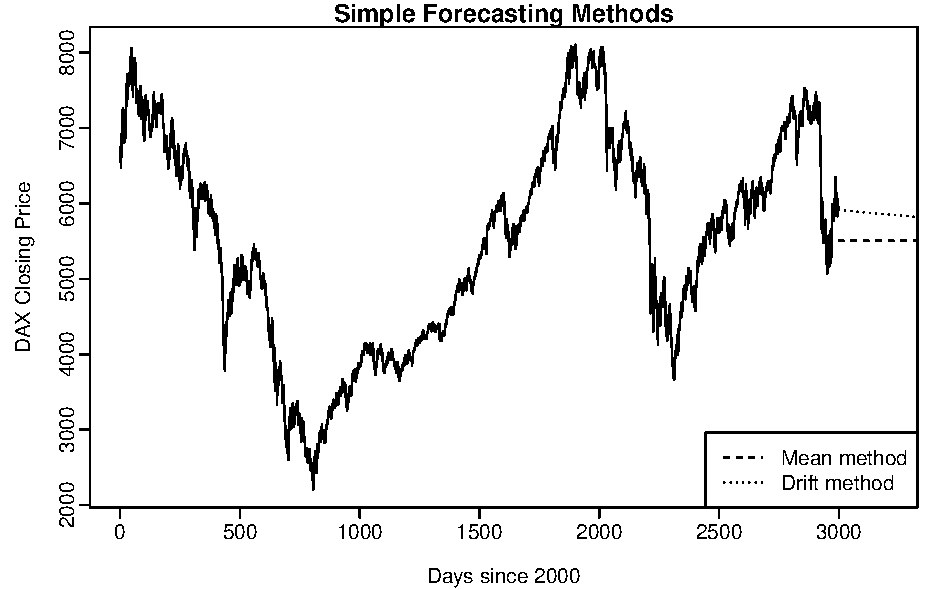
\includegraphics{Figures/chp_ts_dax1}
\caption[Results of simple modelling methods.]{Results of simple modelling methods.}
\label{fig:chp5_ts_dax}
\end{figure}

Figure \ref{fig:chp5_ts_dax_act} is the same as Figure \ref{fig:chp5_ts_dax} except the actual data encountered during the foecast period has been added.

\begin{figure}[tbh]
\centering
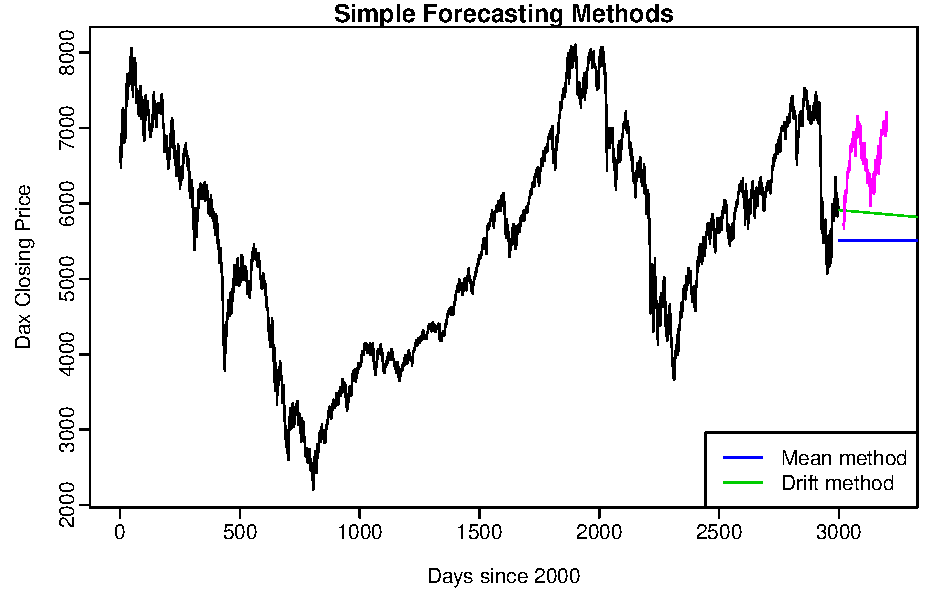
\includegraphics{Figures/chp_ts_dax1_plus_act_data}
\caption[Results of simple modelling methods and actual data.]{Results of simple modelling methods with actual data in forecast period added.}
\label{fig:chp5_ts_dax_act}
\end{figure}

\section{Exponential Smoothing}

Using Rob J Hyndman's forecast package and the ets() function, a variety of exponential smoothing methods can be applied to sample data \citep{Hyndman08automatictime}. Table \ref{tab:tax_em} lists fifteen possibilities when one combines trend and seasonality. In fact Hyndman extends this further by allowing the error term to be either added or multiplied against the results. 

\begin{table}[ht]
\centering
\caption[Taxonomy of exponential smoothing methods.]{of exponential smoothing methods.} 
\label{tab:tax_em}
\begin{tabular}{lccc}
  \toprule 
            & \multicolumn{3}{c}{Seasonal Component} \\
  \cmidrule(r){2-4}
  Trend     & N      & A          & M       \\ 
  Component &(None)  &(Additive)  & (Multiplicative)  \\
  \midrule 
  N (None) & (N,N)&(N,A)&(N,M)  \\ 
  A (Additive) & (A,N)&	(A,A)&(A,M)  \\ 
  Ad (Additive damped) &(Ad,N)&(Ad,A)&(Ad,M) \\ 
  M (Multiplicative) &(M,N)&(M,A)&(M,M)  \\ 
  Md (Multiplicative damped) &(Md,N)&(Md,A)&(Md,M) \\ 
   \bottomrule \end{tabular}
\end{table}

Note - Hymndman: hard to beat the ets model, 37 mins.


% ------ NEW PAGE --------------------------
\newpage
\section{ARIMA}

Figure \ref{fig:chp_ts_rm_arima} shows the Rapid Miner process used to generate Arima models. The various components are as follows:

\begin{itemize}
\item Read CSV - reads in the appropriate data set.
\item Select Attribute (1) - selects the attribute that will be processed in the following steps.
\item Rename - renames the attribute selected in Select Attribute (1) to \textquotedblleft attr1" which is then used in the est of the steps. This component is used to make it easy to change the attribute without having to rename all the subsequent steps.
\item Moving Average - calculates a moving average of the time series (see section \ref{sec:chp2_sma} for details.) This provides the q in ARIMA(p,d,q) models.
\item Differentiate - calculates the difference in the time series and provides the d in ARIMA(p,d,q) models.
\item Lag - creates lag variables which are values of the attribute (the attribute itself, the moving average or the difference value) at earlier points in the time series.
\item Select Attribute (2) - selects the attributes that will be passed to the validation block. Attributes regaring today's values are removed because we are building a model to calculate them and don't want to \textquotedblleft peak" at them before the model is built.
\item Set Role - sets an attribute as the label to be predicted.

\end{itemize}

\begin{figure}[!tbh]
\centering
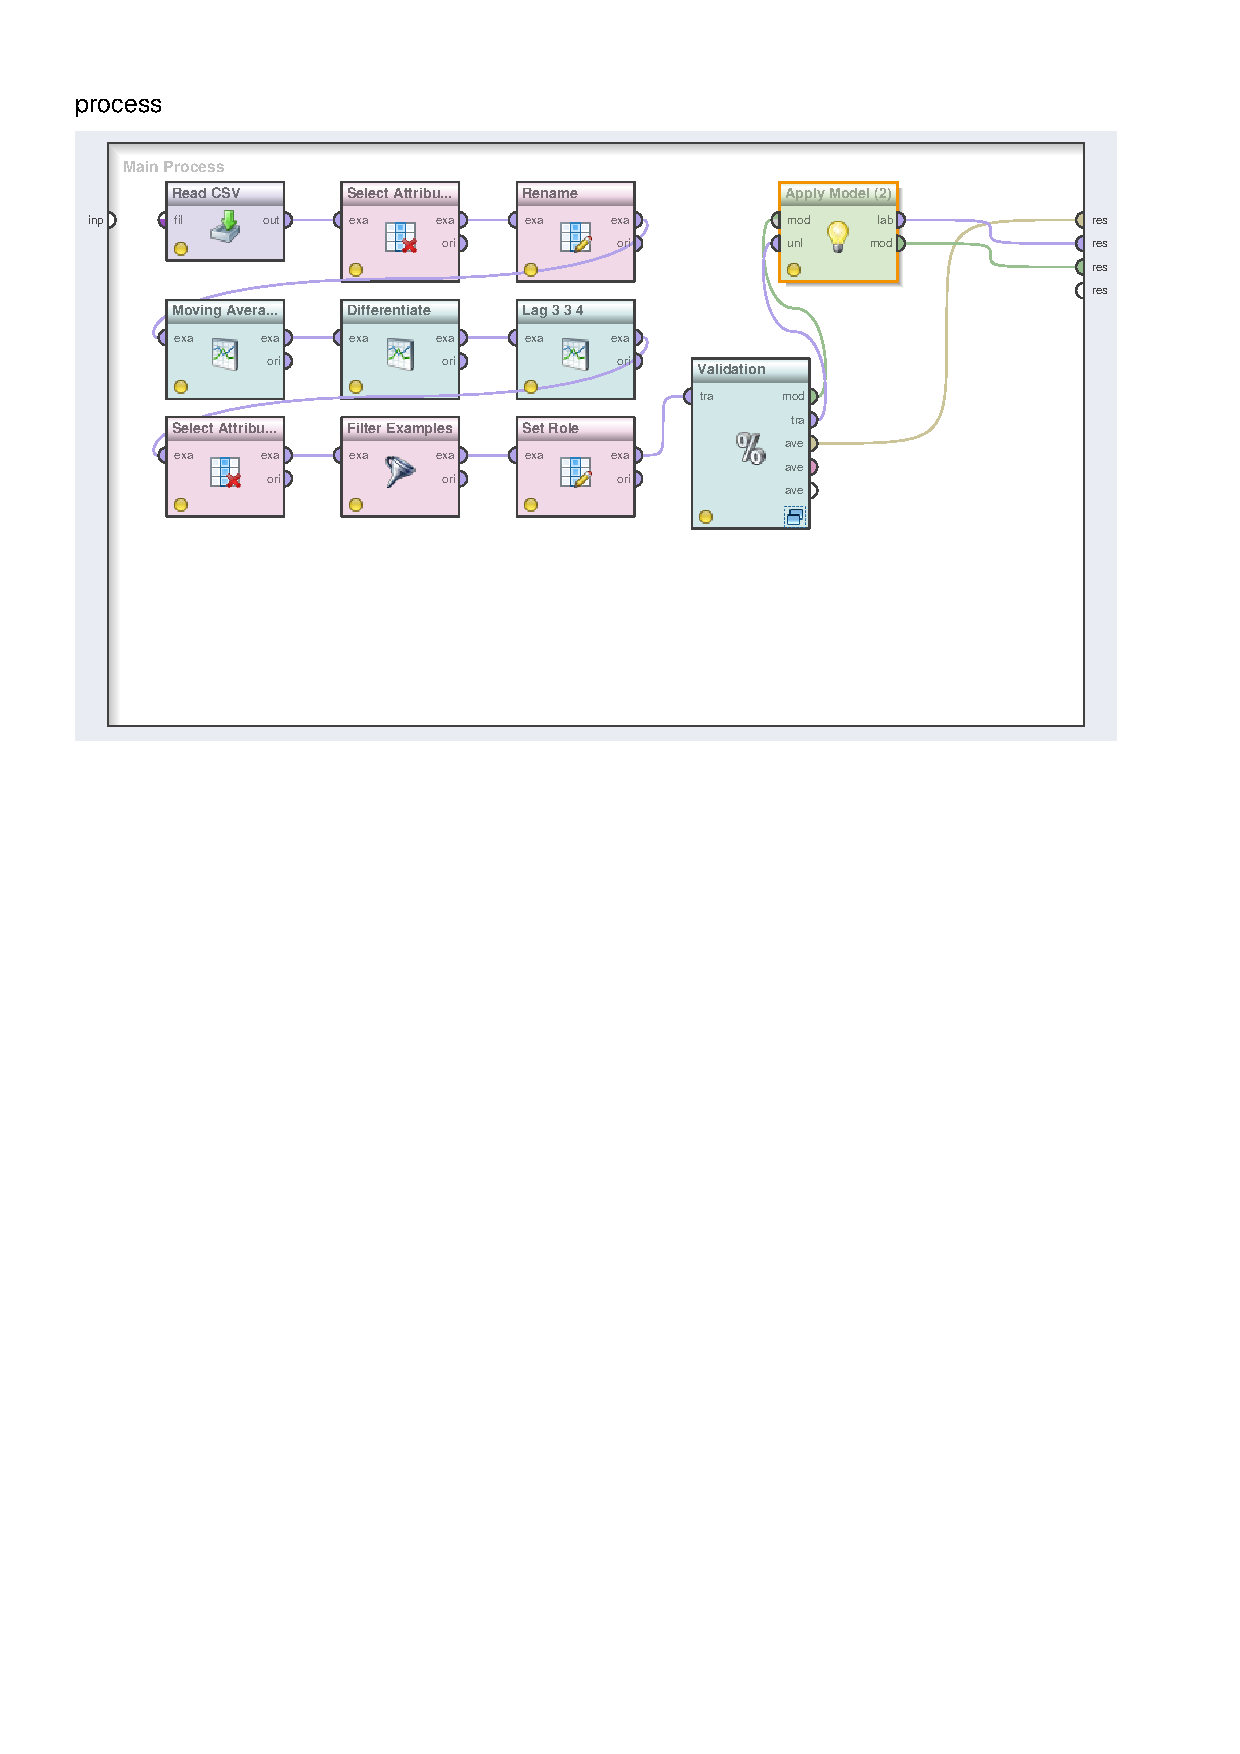
\includegraphics[width=12cm]{../Figures/chp_ts_rm_arima}
\caption[Rapid Miner Arima Process]{Rapid Miner Arima Process.}
\label{fig:chp_ts_rm_arima}
\end{figure}

Questions - should we pass the diff values ot the model - just to flatten the series?

TO DO - auto forecast - on window - does model change? prediction any good? ets and arima ...


